\chapter{CouchDB}

\begin{wrapfigure}{l}{0.3\textwidth}
  \vspace{-110pt}
  \begin{center}
    
\includegraphics[width=0.28\textwidth]{couch.png}
  \end{center}
  \vspace{-70pt}
\end{wrapfigure}
Apache CouchDB, commonly referred to as CouchDB, is an open source database that focuses on ease of use and on being <<a database that completely embraces the web>>. It is a NoSQL database that uses JSON to store data, JavaScript as its query language using MapReduce and HTTP for an API.

\section{Short specification}

\begin{itemize}
  \item \textbf{Written in:} Erlang
  \item \textbf{Main point:} DB consistency, ease of use
  \item \textbf{License:} Apache License 2.0
  \item \textbf{Protocol:} HTTP/REST
  \item \textbf{Web site:} \href{http://couchdb.apache.org/}{couchdb.apache.org}
\end{itemize}

\section{Main features}

\begin{figure}[hb]
  \centering
  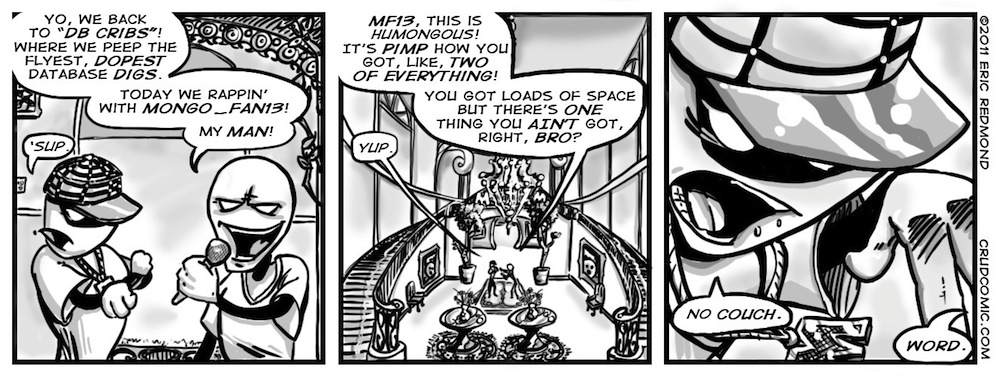
\includegraphics[width=1\textwidth]{couch_vs_mongo.jpeg}
\end{figure}

\subsection{Document Storage}

All documents stores in JSON format, so schema of records is flexible, like in MongoDB.

\subsection{Document Revisions}

All documents have list of revisions (old versions of this document), this can help do rollback of documents.

\subsection{Map/Reduce Views and Indexes}

The data stored is structured using views. In CouchDB, each view is constructed by a JavaScript function that acts as the Map half of a map/reduce operation. The function takes a document and transforms it into a single value which it returns. CouchDB can index views and keep those indexes updated as documents are added, removed, or updated.

\subsection{REST API}

CouchDB stored all items as a resources, each have unique URI and you can do CRUD (Create, Read, Update, Delete) operations on all resources.

\subsection{CouchApp}

Because of the architecture CouchDB is built on, it is actually possible to build entire web applications that reside inside an CouchDB database. We call these applications CouchApps. CouchApps allow you to create full database-driven applications using nothing but HTML5, CSS and JavaScript. The beauty of these apps is that they allow you to take full advantage of CouchDB's powerful replication features to replicate your CouchApp across CouchDB instances. This allows you to keep your CouchApp on several devices, and synchronize them, with automated incremental replication keeping your data up-to-date on each device. Exists CouchApp, which written on Python\footnote{http://couchapp.org} and written on Node.js\footnote{https://github.com/mikeal/node.couchapp.js}.

\subsection{Distributed Architecture with Replication}

CouchDB was designed with bi-direction replication (or synchronization) and off-line operation in mind. That means multiple replicas can have their own copies of the same data, modify it, and then sync those changes at a later time. The biggest gotcha typically associated with this level of flexibility is conflicts.

\subsection{Eventual Consistency}

CouchDB guarantees eventual consistency to be able to provide both availability and partition tolerance.

\section{Strengths}

CouchDB is a robust and stable member of the NoSQL community. Built on the philosophy that networks are unreliable and hardware failure is imminent, CouchDB offers a heartily decentralized approach to data storage. Small enough to live in your smartphone and big enough to support the enterprise, CouchDB affords a variety of deployment situations.

CouchDB is as much an API as a database. In this chapter, we focused on the canonical Apache CouchDB project, but there are an increasing number of alternative implementations and CouchDB service providers built on hybrid back ends. Because CouchDB is made <<of the Web, for the Web,>> it’s fairly straightforward to layer in web technologies~-- such as load balancers and caching layers~-- and still end up with something that’s true to CouchDB’s APIs.\cite{seven_databases}

\section{Weaknesses}

Of course, CouchDB isn’t for everything. CouchDB's mapreduce-based views, while novel, can't perform all the fancy data slicing you'd expect from a relational database. In fact, you shouldn’t be running ad hoc queries at all in production. Also, CouchDB's replication strategy isn't always the right choice. CouchDB replication is all or nothing, meaning all replicated servers will have the same contents. There is no sharding to distribute content around the datacenter. The principal reason for adding more CouchDB nodes is not to spread the data around so much as to increase throughput for read and write operations.\cite{seven_databases}

\section{Tips}

\subsection{Filtering Views by Parts of a Complex Key}

In CouchDB, the sorting of view results is based upon the key. In some cases, you need only filter by the first part of complex key. For example, the last part of keys used for ordering (in my practical work with CouchDB such possibility is often required). You need to select ordered data by keys [user\_id, group\_id, timestamp] and you have only user\_id and group\_id.

Thanks Ryan Kirkman for his article\cite{couchdb_filtering_views}, in which he show how to solve such a problem. You have to use <<startkey>> and <<endkey>> if you want to filter by part of a complex key. If you want to filter using just <<key>> all parts of the complex key must be specified or you will get a null result, as <<key>> is looking for an exact match.

Note that when filtering by part of the complex key, you can only filter by in-order combinations. For example, if you had [field1, field2, field3] as a key, you could only filter by [field1], [field1, field2] or [field1, field2, field3]. You could not, for example, filter by [field1, field3], as CouchDB would interpret the key you specified for field3 as the value to filter field2 by.

The syntax required to use startkey=\dots\&endkey=\dots~when you want to filter on only part of a complex key is as follows:
Say we had a key like [user\_id, group\_id, timestamp], and we wanted to filter on only user\_id and group\_id where user\_id=123 and group\_id=456. Our url would look like:

\begin{lstlisting}
http://localhost:5984/database/_design/app/
_view/messages?startkey=[123, 456]&endkey=[123,456,{}]
\end{lstlisting}

Notice the <<\{\}>> in the <<endkey>>. This is so that we get all values returned by the view between <<null>> and <<\{\}>>, which for just about every case should be everything.

\subsection{Rebuilding of views}

Before CouchDB version 1.1.0 there was a small problem existing. View was automatically rebuilt on every request. If you have a huge number of documents, then such operation takes a long time. To solve this problem, a <<stale=ok>> parameter was proposed. It returns last built view results without rebuilding (of course, on first request it will still build view results). In this case, you need to reset cached view results by crontab or find another way for this. Starting from version 1.1.0 a new parameter called <<stale=update\_after>> exists. It provides the same effect as <<stale=ok>>, but the view rebuilds automatically after response.

\subsection{Use the native reduce functions written on Erlang}

Do not reinvent the wheel. You can find such code in the documentation as an example:

\begin{lstlisting}[language=Javascript]
function (key, values, rereduce) {
   return sum(values);
}
\end{lstlisting}

Try to avoid them and use the native reduce functions written on Erlang: <<\_count>> and <<\_sum>>, which also operate faster than Javascript analogs.

\subsection{Use more databases}

In many books for beginners (including CouchDB: The Definitive Guide\footnote{http://guide.couchdb.org/}) examples looks very nice, but it isn’t combined with real life. As soon as the number of your document grows the development of temporary views becomes almost impossible, because the server now needs to go through all your documents for compliance with the map-function. The logic of CouchDB is following: when you update a document in the database~-- it affects all documents. Therefore, completely all documents update their ETag when updating just a single document. This is one disadvantage in using many documents from various fields. At the same time, update of a document does not affect the ETag of other documents, because the ETag of documents is their latest revision. Solving these problems help division of documents (by types or another logical structures) by databases.

\subsection{Cache data using the ETag}

Receiving data from CouchDB with headers <<If-Modified-Since/ETag>> is really a fast data retrieval. Do not forget that when you use headers <<If-None-Match>>, with response status 304 response body is always empty, because the server assumes that you are storing data.

Each update of the document leads to the creation of its newer revision. Also, this leads to the rebuild of views, in which this document is used (on addition and removal of documents also rebuild views) in their next call. All old revisions are saved, and not always you need to have all document revisions. Database size is growing, so don't forget to perform the operation for the compaction of all documents. This saves a lot of free disk space.

\subsection{Full-text search}

CouchDB is suitable for many tasks, but not for all. Full-text search falls under this exception. Since we can not pass a parameter directly in a view, we cannot find anything like in the database. So you will not be able to organize a search on the site using CouchDB. To solve this problem~-- use a separate search engine. There are already solutions like Lucene (connected by couchdb-lucene) and Elasticsearch (with a plugin for CouchDB) exists.

\subsection{Geo search}

Another problem in CouchDB is a geo search, for example, find all objects within N miles. In SQL-like database, this task is implemented using a small function that allows to determine the distance between two points by latitude and longitude. In CouchDB, we have only one scale sorting keys, so finding all the points that fall into the square~-- almost impossible. Almost~-- means having exist solution isn’t perfect. Geo search can be implemented by Geohash\footnote{http://en.wikipedia.org/wiki/Geohash}\footnote{https://github.com/davetroy/geohash-js}. The implementation is that any position on a map can be represented as a numeric-literal hash. At the same time, rather than the specified coordinates, the greater the length of the hash. Thus, you can transfer geohash as the key and to vary its length in the parameters startkey/endkey to refine the search radius (of course this is not the radius).


\section{Use cases}

\begin{itemize}
  \item CRM, CMS systems
  \item S3-like services
  \item Cloud infrastructure
  \item Scalable, low-latency storage for mobile apps
  \item Financial applications (where need full history of record changes)
\end{itemize}